% This file was created by tikzplotlib v0.9.1.
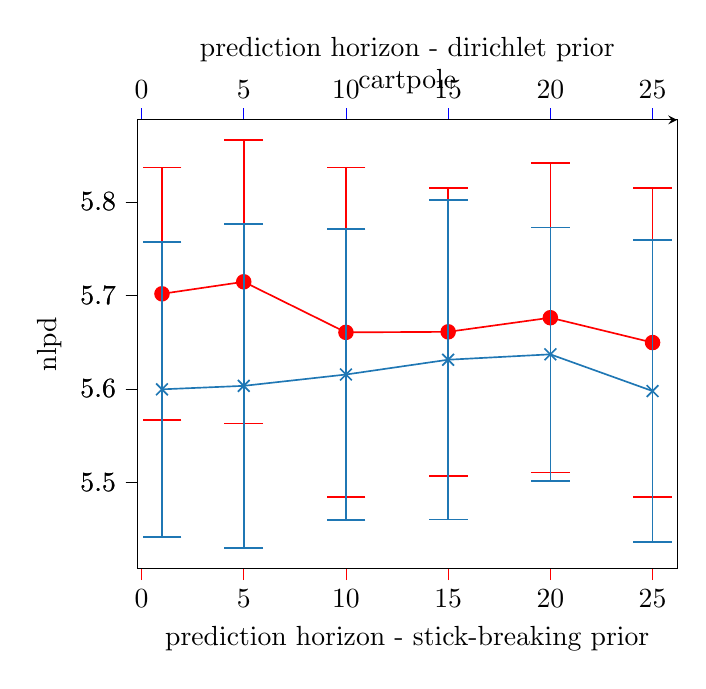
\begin{tikzpicture}

\definecolor{color0}{rgb}{0.12156862745098,0.466666666666667,0.705882352941177}

\begin{axis}[
tick align=outside,
tick pos=left,
title={cartpole},
x grid style={white!69.0196078431373!black},
xlabel={prediction horizon - stick-breaking prior},
xmin=-0.2, xmax=26.2,
xtick style={color=red},
y grid style={white!69.0196078431373!black},
ylabel={nlpd},
ymin=5.40831279956981, ymax=5.88782115480196,
ytick style={color=black},
ytick={5.4,5.5,5.6,5.7,5.8,5.9},
yticklabels={5.4,5.5,5.6,5.7,5.8,5.9}
]
\path [draw=red, semithick]
(axis cs:1,5.56655285919505)
--(axis cs:1,5.83709420224589);

\path [draw=red, semithick]
(axis cs:5,5.56329462680099)
--(axis cs:5,5.86602532047322);

\path [draw=red, semithick]
(axis cs:10,5.48424833952041)
--(axis cs:10,5.83693606107872);

\path [draw=red, semithick]
(axis cs:15,5.50729816626637)
--(axis cs:15,5.81502329766467);

\path [draw=red, semithick]
(axis cs:20,5.51087812957063)
--(axis cs:20,5.84165602536383);

\path [draw=red, semithick]
(axis cs:25,5.48443890222786)
--(axis cs:25,5.81493101517007);

\addplot [semithick, red, mark=-, mark size=7, mark options={solid}, only marks]
table {%
1 5.56655285919505
5 5.56329462680099
10 5.48424833952041
15 5.50729816626637
20 5.51087812957063
25 5.48443890222786
};
\addplot [semithick, red, mark=-, mark size=7, mark options={solid}, only marks]
table {%
1 5.83709420224589
5 5.86602532047322
10 5.83693606107872
15 5.81502329766467
20 5.84165602536383
25 5.81493101517007
};
\addplot [semithick, red, mark=*, mark size=2.5, mark options={solid}]
table {%
1 5.70182353072047
5 5.71465997363711
10 5.66059220029956
15 5.66116073196552
20 5.67626707746723
25 5.64968495869897
};
\end{axis}

\begin{axis}[
axis x line=top,
tick align=outside,
x grid style={white!69.0196078431373!black},
xlabel={prediction horizon - dirichlet prior},
xmin=-0.2, xmax=26.2,
xtick pos=right,
xtick style={color=blue},
y grid style={white!69.0196078431373!black},
ymin=5.40831279956981, ymax=5.88782115480196,
ytick pos=left,
ytick style={color=black}
]
\path [draw=color0, semithick]
(axis cs:1,5.44200097342462)
--(axis cs:1,5.75732738022257);

\path [draw=color0, semithick]
(axis cs:5,5.43010863389855)
--(axis cs:5,5.77666845176065);

\path [draw=color0, semithick]
(axis cs:10,5.46010231114236)
--(axis cs:10,5.77090221358999);

\path [draw=color0, semithick]
(axis cs:15,5.46060506900209)
--(axis cs:15,5.80203563512146);

\path [draw=color0, semithick]
(axis cs:20,5.50136228142923)
--(axis cs:20,5.77280804230152);

\path [draw=color0, semithick]
(axis cs:25,5.43608570029995)
--(axis cs:25,5.7595464898762);

\addplot [semithick, color0, mark=-, mark size=7, mark options={solid}, only marks]
table {%
1 5.44200097342462
5 5.43010863389855
10 5.46010231114236
15 5.46060506900209
20 5.50136228142923
25 5.43608570029995
};
\addplot [semithick, color0, mark=-, mark size=7, mark options={solid}, only marks]
table {%
1 5.75732738022257
5 5.77666845176065
10 5.77090221358999
15 5.80203563512146
20 5.77280804230152
25 5.7595464898762
};
\addplot [semithick, color0, mark=x, mark size=3, mark options={solid}]
table {%
1 5.5996641768236
5 5.6033885428296
10 5.61550226236617
15 5.63132035206177
20 5.63708516186538
25 5.59781609508808
};
\end{axis}

\end{tikzpicture}
